\documentclass{mcmthesis}
%\usepackage[justification=center]{caption}%表格标题居中
\usepackage{booktabs}%粗表格

\usepackage{indentfirst}%首行缩进
\usepackage{graphicx}%图片
\usepackage{subfigure}

\mcmsetup{tcn = 85691,problem = B,titlepage = false}
\title{Use Diffusion Models to Solve the Problem of Language Communication}
\begin{document}

\setlength{parindent}{2em}%设置段首行缩进2字符

  \begin{abstract}
    This is an example of the ABSTRACT.
  \end{abstract}

  \maketitle
  \tableofcontents

  \section{Introduction}%引言

    \subsection{Terminology}%术语

    \begin{table}[h]
    \centering
    \caption{Notation}

    \begin{tabular}{cc}
    \toprule
    Symbol&Meaning\\
    \midrule
    {$C_1$}&ta\\
    \bottomrule
    \end{tabular}
  \end{table}
    \subsection{Assumptions}%假定

  \section{The Models}


    \subsection{Language Diffusion Model}%语言扩散模型
    \subsubsection{Traditional Diffusion: Fick's Second Law}%传统扩散:菲克第二定律

    Fick's law is a quantitative formula developed by Fick in 1858
    with reference to the Fourier heat conduction equation
    to describe the migration of substances
    from a high concentration region to a low concentration region.
    Fick's second law describes the state as follows
    when the concentration of diffusate varies with time at any point in the diffusion medium,
    that is, the distribution of concentration gradients throughout the system is dynamic:
    $$\frac{\partial C}{\partial t}=D\frac{\partial^2C}{\partial x^2}$$

    Where $C$ is the concentration, $x$ is the coordinate, and $t$ is the time.

    It gives a mathematical expression of the diffusion of matter in the medium.
    We use it to calculate the concentration of each point,
    and integral it to calculate the amount of material.

    $D$ is called the diffusion coefficient.
    It is related to the physical properties of diffusion media and dispersions.
    And it is also a decisive factor in determining the speed of proliferation.
    The larger the $D$, the greater the rate of diffusion.
    \subsubsection{Transform It into the Language Diffusion Model}%将扩散模型转化到语言扩散模型

    Firstly we use a plane to refer to the entire human possession of space.
    We think the area of this plane is limited, and the area is equal to the total human population.
    Of course, this area is also changing
    Then the person who uses the A language is a circle in the center of the plane.
    The area of this circle is the total number of people who use the A language (including the first language and the second language).
    Refer to Picture 1.
    %\ref{p1}

    The expansion of the total number of languages is the process of increasing color.
    In the model, it is the color slowly from the color circle into the plane of the blank, like ink dripping into water slowly spread the same.
    Please note here that the boundary of the circle after diffusion becomes unclear.
    In order to achieve the model's computability, we define a parameter $k$.
    For example: $k=60\%$.
    Take a ring with a color concentration of 60% as a circle border.
    Integrate this ring from the original color circle boundary to the new one.
    We get the number of people who have proliferated.
    This number is an increase in the number of second language
    (Changes in the number of speakers in the first language are related to changes in the population that mainly use the language.)
    This diffusion process is governed by two factors: the circumference of the initial color circle and the rate of diffusion.

    \begin{figure}[h]
      \begin{minipage}[t]{0.5\linewidth}
      \centering
      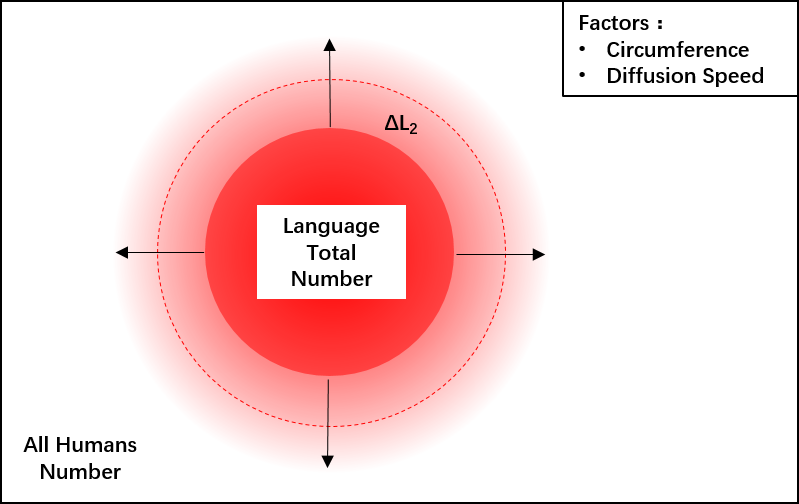
\includegraphics[height=3.8cm,width=6cm]{p1.png}%height=2.4cm,width=3.8cm
      \caption{Language Diffusion Model}
      \label{p1}
      \end{minipage}
      \begin{minipage}[t]{0.5\linewidth}
      \centering
      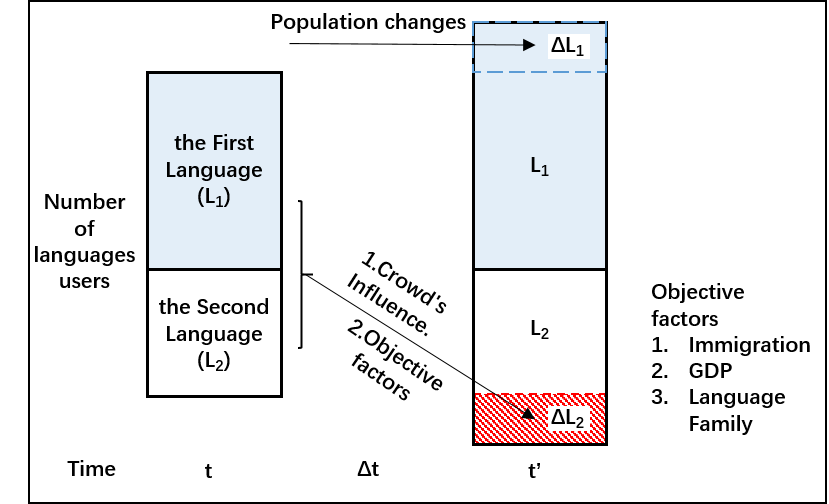
\includegraphics[height=3.8cm,width=6.3cm]{p2.png}%width = .48\linewidth
      \caption{Changing Way in Users}
      \label{p2}
      \end{minipage}
    \end{figure}

    %\begin{figure}
      %\centering
      %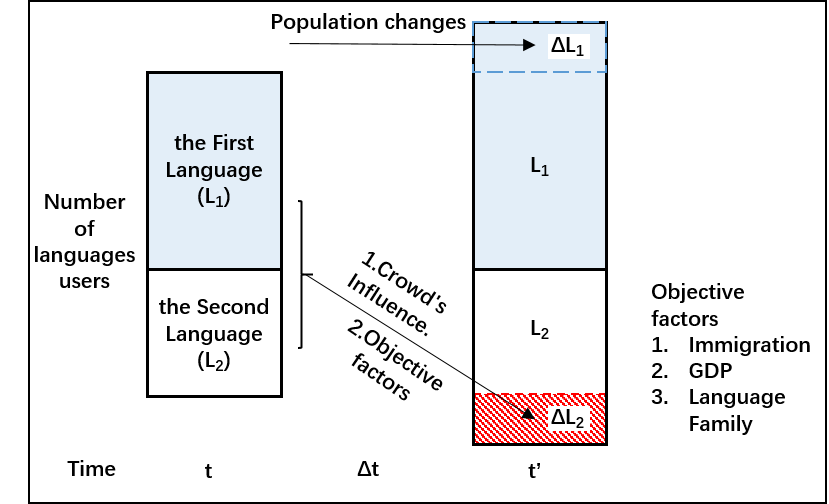
\includegraphics{p2.png}
      %\caption{Changing Way in Users}
      %\label{p2}
    %\end{figure}

    The total number of language changes is divided into two parts, one is the number of changes in the first language, another is the number of changes in the second language.
    Whether it is studying immigrants, work or government incentives, are only increased the number of second languages.
    Therefore, the number of first languages is only related to the growth of the population of many countries that mainly use this language.
    The growth of a second language is related to the overall influence of the language, including the number of people using the language and the objective factors.
    Then the number of users, the larger the corresponding area, the greater the side length.
    This indicator quantifies the crowd's influence.
    Objective factors determine the speed of diffusion.
    We use the diffusion coefficient $D$ to quantify it.
    Furthermore, we analyze the GDP, linguistic systems and the impact of immigrants on the diffusion coefficient in the major countries that use languages.
    This represents the degree to which people in real life learn the language.
    Refer to Picture 2.

    As the number of languages used is too large (hundred million),
    the effect of the number of people who grew over time on the radius of the circle is negligible.
    At this point we can approximate the ring as a rectangle.
    We do not consider differences in proliferation in all directions.
    Then we can calculate the diffusion effect of a line,
    and then multiply the circumference of the original color circle
    to get the number of people added, that is, the " Concentration Area " of the circle.
    "Concentration Area" means that the coloring of this ring is not uniform.
    The actual area is not equivalent to the actual number.
    Take the proportion of people who use the A language per unit area as the concentration $C$.
    Refer to Picture 3.

    \begin{figure}[h]
          \centering
          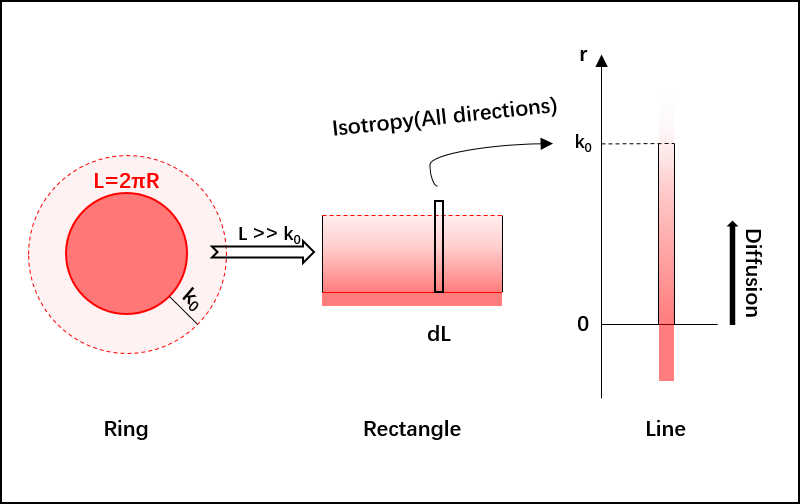
\includegraphics{p3.png}
          \caption{Approximate Replacement Process}
          \label{p3}
        \end{figure}

    Here we solve this situation.
    Fick's second law is a partial differential equation.
    We try to turn it into an ordinary differential equation.
    We suppose that the concentration of the colored circles is constant and then deduced:
    \\Initial conditions: \ \ \ \ \  When \ \ \ $t=0$\ ,\ $x\approx 0$,\ $C_{(x,t)}=0$
    \\Boundary conditions: When \ \ \ \ $t>0$\ ,\ $C_{(0,t)}=1$%\textgreater
    \\Using Boltzmann transformation:
    $$\lambda=\frac{x}{\sqrt{t}}$$
    Substitute Fick's second law:
    $$-\lambda\frac{{\rm d}C}{{\rm d}\lambda}=2D\frac{{\rm d}^2C}{{\rm d}\lambda^2}$$
    After substitution, suppose $\beta=\frac{\lambda}{2\sqrt{D}}=\frac{x}{2\sqrt{Dt}}$ ,
    the result of the final integration is:
    $$C_{(x,t)}=a\int_0^\beta exp(-\beta)^2{\rm d}\beta+b$$
    The integral $\int_0^\beta exp(-\beta)^2{\rm d}\beta$ is called Gaussian error function.
    According to Gaussian error function:
    $$\int_0^\infty exp(-\beta)^2{\rm d}\beta=\frac{\sqrt{\pi}}{2}$$
    Consider initial conditions and boundary conditions:
    \\When $x\rightarrow\infty$,\ then $\beta\rightarrow 0$,\ $C_{(\infty,t)}=a\frac{\sqrt{\pi}}{2}+b=0$
    \\$x=0$,\ then $\beta=0$,\ $C_{(0,t)}=b=1$,then:
    $$a=-\frac{2}{\sqrt{\pi}},b=1$$

    The final concentration equation is:
    $$C_{(x,t)}=1-\frac{2}{\sqrt{\pi}}\int_0^\beta exp(-\beta)^2{\rm d}\beta=1-erf(\frac{x}{2\sqrt{Dt}})$$

    In our model,\ $r$ represents the distance to the colored circle border.
    So we replace $r$ with $x$ :
    $$C_{(r,t)}=1-erf(\frac{r}{2\sqrt{Dt}})$$
    We integrate this concentration function.
    As mentioned earlier, in order for the results to be presented, we agree on a ratio $k$.
    The ring of concentration $k$ is the upper bound of the integral.
    $k$ corresponding to the distance k0 obtained by the formula:$C_{(k_0,t)}=k$
    \\Then the final increment of the second language ($\Delta L_2$) is expressed as:
    Concentration Integral × Colored Circle Circumference
    $$\Delta L_2=\int_0^{k_0} C_{(r,t)}{\rm d}r\times 2\pi\sqrt{\frac{T}{\pi}}=\int_0^{k_0}(1-erf(\frac{r}{2\sqrt{Dt}})){\rm d}r\times 2\pi\sqrt{\frac{T}{\pi}}$$





    \subsection{Design of Influential Factors}%语言传播的影响因素
    A large number of objective factors will affect the spread of language.








\end{document}
